\documentclass[tikz,border=2pt]{standalone}
\usepackage{tikz}
\usetikzlibrary{arrows.meta,positioning,fit,backgrounds,calc}
\definecolor{blue}{HTML}{0072B2}
\definecolor{sky}{HTML}{56B4E9}
\definecolor{green}{HTML}{009E73}
\definecolor{orange}{HTML}{E69F00}
\definecolor{verm}{HTML}{D55E00}
\definecolor{ink}{HTML}{263238}
\definecolor{paper}{HTML}{F5F7F8}
\begin{document}
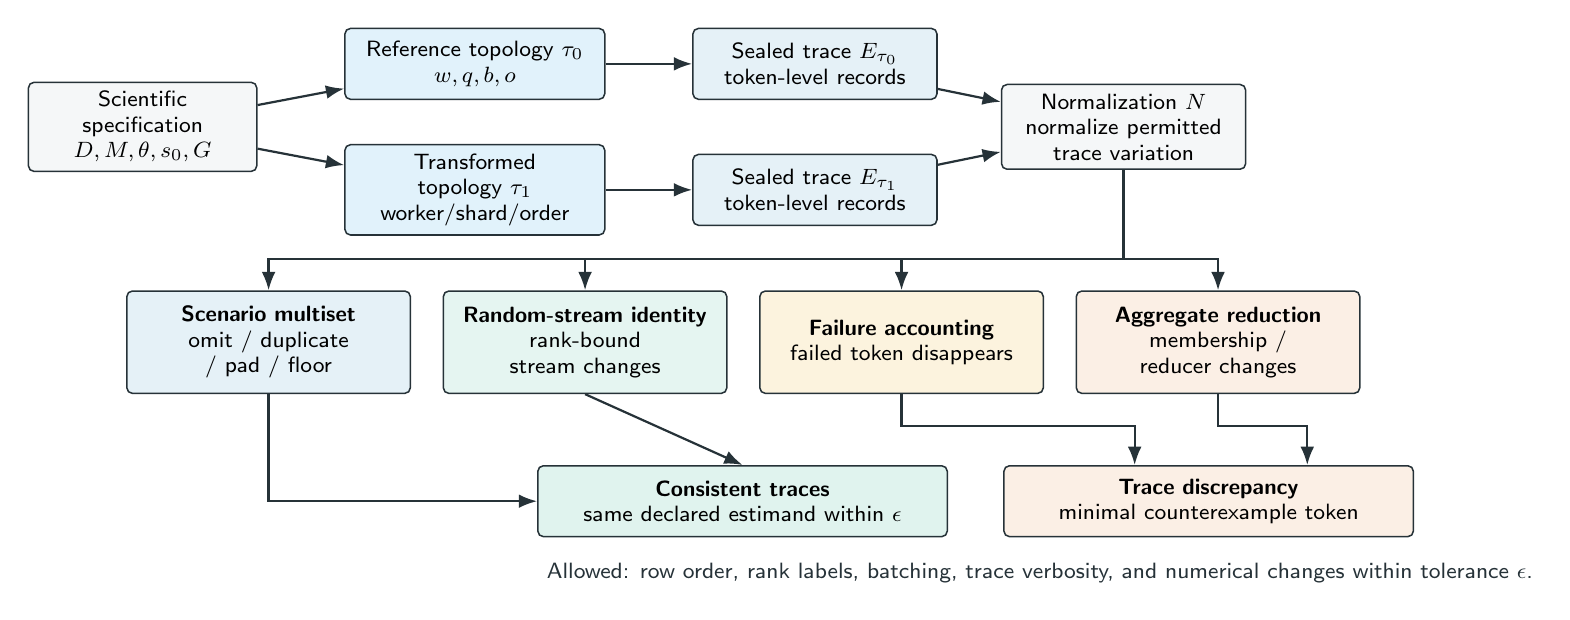
\begin{tikzpicture}[font=\sffamily\fontsize{8}{9.2}\selectfont,>=Latex,
  box/.style={draw=ink,rounded corners=2pt,minimum height=9mm,align=center,fill=white,line width=.55pt},
  flow/.style={-Latex,line width=.8pt,draw=ink},
  rel/.style={box,minimum width=36mm,minimum height=13mm,text width=32mm},
  small/.style={font=\sffamily\fontsize{8}{9}\selectfont}]
\node[box,fill=paper,minimum width=29mm,text width=25mm] (spec) {Scientific specification\\$D,M,\theta,s_0,G$};
\node[box,fill=sky!18,minimum width=33mm,text width=29mm,right=11mm of spec,yshift=8mm] (t0) {Reference topology $\tau_0$\\$w,q,b,o$};
\node[box,fill=sky!18,minimum width=33mm,text width=29mm,right=11mm of spec,yshift=-8mm] (t1) {Transformed topology $\tau_1$\\worker/shard/order};
\node[box,fill=blue!10,minimum width=31mm,text width=27mm,right=11mm of t0] (e0) {Sealed trace $E_{\tau_0}$\\token-level records};
\node[box,fill=blue!10,minimum width=31mm,text width=27mm,right=11mm of t1] (e1) {Sealed trace $E_{\tau_1}$\\token-level records};
\node[box,fill=paper,minimum width=31mm,text width=27mm,right=2.36cm of $(e0)!0.5!(e1)$] (norm) {Normalization $N$\\normalize permitted\\trace variation};
\draw[flow] (spec) -- (t0); \draw[flow] (spec) -- (t1);
\draw[flow] (t0) -- (e0); \draw[flow] (t1) -- (e1);
\draw[flow] (e0) -- (norm); \draw[flow] (e1) -- (norm);

\node[rel,fill=blue!10,below=15mm of spec,xshift=16mm] (scenario) {\textbf{Scenario multiset}\\omit / duplicate / pad / floor};
\node[rel,fill=green!10,right=4mm of scenario] (randomstream) {\textbf{Random-stream identity}\\rank-bound stream changes};
\node[rel,fill=orange!13,right=4mm of randomstream] (failureaccounting) {\textbf{Failure accounting}\\failed token disappears};
\node[rel,fill=verm!10,right=4mm of failureaccounting] (aggregation) {\textbf{Aggregate reduction}\\membership /\\reducer changes};
\coordinate (mid) at ($(randomstream.north)!0.5!(failureaccounting.north)$);
\draw[flow] (norm.south) |- ([yshift=4mm]mid) -| (scenario.north);
\draw[flow] ([yshift=4mm]mid) -| (randomstream.north);
\draw[flow] ([yshift=4mm]mid) -| (failureaccounting.north);
\draw[flow] ([yshift=4mm]mid) -| (aggregation.north);

\node[box,fill=green!12,minimum width=52mm,text width=48mm,below=9mm of randomstream,xshift=20mm] (consistent) {\textbf{Consistent traces}\\same declared estimand within $\epsilon$};
\node[box,fill=verm!10,minimum width=52mm,text width=48mm,right=7mm of consistent] (discrepancy) {\textbf{Trace discrepancy}\\minimal counterexample token};
\draw[flow] (scenario.south) |- (consistent.west); \draw[flow] (randomstream.south) -- (consistent.north);
\coordinate (discrepancyleft) at ($(discrepancy.north west)!0.32!(discrepancy.north east)$);
\coordinate (discrepancyright) at ($(discrepancy.north west)!0.74!(discrepancy.north east)$);
\draw[flow] (failureaccounting.south) -- ++(0,-4mm) -| (discrepancyleft);
\draw[flow] (aggregation.south) -- ++(0,-4mm) -| (discrepancyright);
\node[small,anchor=north west,text=ink] at ([yshift=-2mm]consistent.south west) {Allowed: row order, rank labels, batching, trace verbosity, and numerical changes within tolerance $\epsilon$.};
\end{tikzpicture}
\end{document}
